\nnarticleheader{Four Proofs of Euler's Identity}{Elise Kait, Baldwin ‘21}
Discovered by Swiss mathematician Leonard Euler, the Euler identity is the perfect archetype of mathematical elegance, as it combines 5 of the most fundamental constants in mathematics in a single equation:
\[e^{i\pi}+1=0\]

\noindent
$0 \rightarrow$ the additive identity
\\* $1 \rightarrow$ the multiplicative identity
\\* $e \rightarrow$ Euler’s number ($\sim 2.718$, appears widely in mathematics and underlies exponential growth)
\\* $\pi \rightarrow$ Pi ($\sim$ 3.1415…), relates the radius and circumference of a circle
\\* $i \rightarrow$ the imaginary or complex unit ($\sqrt{-1}$)

Euler’s identity is actually a special case of Euler’s formula...
\[e^{i\theta}=\cos\theta + i\sin\theta\]
...derived by solving the identity at an angle of 180$^{\circ}$, or simply plugging in $\pi$ for the angle $\theta$:
\[e^{i\pi}=\cos(\pi) + i\sin(\pi)\]
\[e^{i\pi}=-1+i(0)=-1\]
\[e^{i\pi}=-1\]
\[e^{i\pi}+1=0\]

This doesn’t really tell us much, so it is important to understand Euler’s formula, which relates Euler’s number, the imaginary unit $i$, and the trigonometric functions sine and cosine. Here, I will show four ways to prove Euler’s formula to fully demonstrate its importance in mathematics.

\noindent
\textbf{Proof 1: Taylor Series Expansion}

The first and most common proof of Euler’s formula uses a Calculus technique, known as a Taylor series, to expand $e^{ix}$. A Taylor series is a way of expressing a non-polynomial function as an infinite sum of polynomials found through derivatives. Three common Taylor series expansions are used to prove Euler’s formula:
\[e^{x}=\sum_{n=0}^{\infty} \frac{x^{n}}{n!}  = 1 + x+ \frac{x^2}{2!} + \frac{x^3}{3!} + \frac{x^4}{4!} + ... + \frac{x^n}{n!}\]
\[\sin x=\sum_{n=0}^{\infty} (-1)^n \frac{x^{2n+1}}{(2n+1)!}  = x - \frac{x^3}{3!} + \frac{x^5}{5!} - \frac{x^7}{7!} + ...\]
\[\cos x=\sum_{n=0}^{\infty} (-1)^n \frac{x^{2n}}{(2n)!}  = 1 - \frac{x^2}{2!} + \frac{x^4}{4!} - \frac{x^6}{6!} + ...\]

Now, we can manipulate the Taylor series for $e^x$,
\[e^x=1+x+\frac{x^2}{2!}+\frac{x^3}{3!}+\frac{x^4}{4!}\frac{x^5}{5!}+\frac{x^6}{6!}+...\]
\[e^{ix}=1+ix+\frac{(ix)^2}{2!}+\frac{(ix)^3}{3!}+\frac{(ix)^4}{4!}+\frac{(ix)^5}{5!}+\frac{(ix)^6}{6!}
+\frac{(ix)^7}{7!}+\frac{(ix)^8}{8!}+...\]
\[=1+ix-\frac{x^2}{2!}-\frac{(ix)^3}{3!}+\frac{x^4}{4!}+\frac{(ix)^5}{5!}-\frac{x^6}{6!}-\frac{(ix)^7}{7!}+\frac{x^8}{8!}+...\] 
\begin{center}(\textit{note that $i^2=-1$})\end{center}
\[=(1-\frac{x^2}{2!}+\frac{x^4}{4!}-\frac{x^6}{6!}+\frac{x^8}{8!}-...)+i(x-\frac{x^3}{3!}+\frac{x^5}{5!}-\frac{x^7}{7!}+...\]
\[=\cos x + i\sin x\]

\noindent
\textbf{Proof 2: Complex Power Computation}

A second way to prove Euler’s formula comes about unintentionally, by computing a number to a complex power.

Let’s look at a table of the successive powers of $10^{\frac{i}{8}}$:

%First image here (source: Feynman, Richard P., et al. Mainly Mechanics, Radiation, and Heat. Addison-Wesley Publishing Company, 1963. [Table 22-4].)

\renewcommand{\thefigure}{1}
\begin{figure}[h]
  \begin{center}
    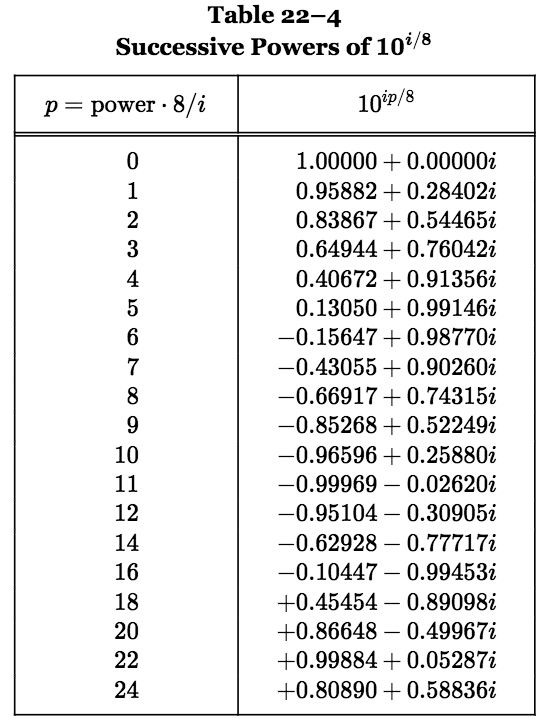
\includegraphics[scale=.55]{kait_image1}
  \end{center}
  \caption{Successive powers of $10^{\frac{i}{8}}$.}
  \label{fig:1}
\end{figure}

(Note: the expression $\frac{ip}{8}$ is simplified to $is$ as a means of denoting some arbitrary constant with which $i$ is multiplied). Looking at these values, we can see that the values seem to oscillate in some way. We should also look at a graph of these numbers where there is one function of the $x$ value and one for the $iy$ value.

%Second image here (source: Feynman, Richard P., et al. Mainly Mechanics, Radiation, and Heat. Addison-Wesley Publishing Company, 1963. [Figure 22-1].)
\renewcommand{\thefigure}{2}
\begin{figure}[h]
  \begin{center}
    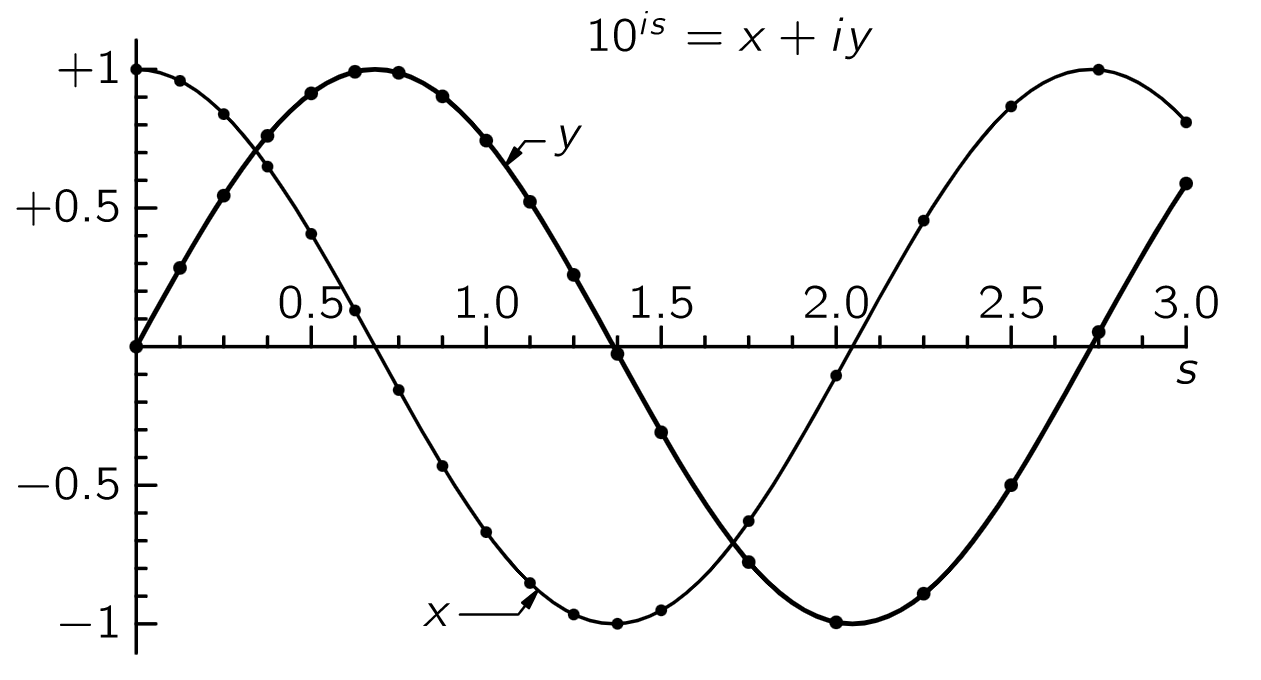
\includegraphics[scale=.23]{kait_image2}
  \end{center}
  \caption{Graph of values from Fig. 1.}
  \label{fig:2}
\end{figure}

\noindent
\textbf{Proof 3: Solution to $\frac{dy}{dx}=iy$}

Euler’s formula solves the first-order differential equation, $\frac{dy}{dx}=iy$.

We get this differential equation from taking the first derivative of $y=e^{ix}$, which is $\frac{dy}{dx}=ie^{ix}$, or, substituting the value of $y$ from the first equation, $\frac{dy}{dx}=iy$. To find a solution, we need a function other than $e^{ix}$ for which $\frac{dy}{dx}=iy$. So we use Euler’s formula:
\[y=\cos x + i\sin x\]
\[\frac{dy}{dx}= -\sin x + i\cos x\]
\[\frac{dy}{dx}= i(i\sin x + \cos x), because \frac{-\sin x}{i}=\frac{1}{i} \cdot \frac{-\sin x}{1} = \frac{i}{i^2} \cdot \frac{-\sin x}{1} = -i \cdot -\sin x = i\sin x\]
\[\frac{dy}{dx} = i(\cos x + i\sin x)\]
\[\frac{dy}{dx} = i(y)\]

This connection between the function $e^{ix}$ and its derivative $ie^{ix}$ is very important and reminds us of Proof 2, in which we discussed the geometric interpretation of the function. $e^x$ itself is arguably the single most important first order differential equation $y’=y$, the only function whose derivative is itself. $e^{ix}$ has a similar importance, but in the realm of complex numbers.

\noindent
\textbf{Proof 4: Geometric Intuition}

I’ve proven Euler’s formula three times now, and while they are each mathematically sound, they give little detail of the true nature of the formula. Euler’s formula must also be understood intuitively using geometry and a complex plane coordinate system, then via two ways to traverse a circle. 

In a geometric sense, Euler’s formula is not so much an input $\rightarrow$ output function, but rather two seperate ways to define a point on the complex plane (the x-axis consists of real numbers, and the y-axis consists of “imaginary” numbers, or multiples of $i$).

%Third image here (source: https://commons.wikimedia.org/wiki/File:Euler%27s_formula.png)
\renewcommand{\thefigure}{3}
\begin{figure}[h]
  \begin{center}
    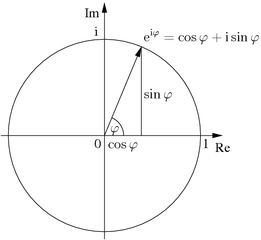
\includegraphics[scale=2]{kait_image3}
  \end{center}
  \caption{The unit circle in the complex plane.}
  \label{fig:3}
\end{figure}

One way to define a point on a circle is by making a triangle whose hypotenuse is the radius and connecting the point on the circle down to an axis. Then, if we know the angle of the radius, we can use sine and cosine to express the lengths of the legs. Any point on the complex unit circle/complex plane can be expressed as such: $(x, iy)$ or as $x+iy$.

For example, $\varphi = \frac{\pi}{2}$ can be expressed as $(0, 1i)$ or $0 + 1i$ since:
\[e^{i\frac{\pi}{2}} = \cos (\frac{\pi}{2}) + i\sin (\frac{\pi}{2})\]
\[=0+1i\]

We can write any complex number on the complex plane using a scalar, $k$:
\[c_1 = k(\cos (\varphi) = i\sin (\varphi))\]
\[= ke^{i\varphi}, k \in \mathbb{R}\]

There is a second way that we can define a point on a complex unit circle involving radians. But first we must understand the difference between exponential growth and complex growth in a complex coordinate system. Real exponential growth ‘pulls’ a number in one direction. For example, as x increases, $2^x=1,2,4,8,16,32,62...$. Each ‘pull’ makes a number get larger and larger, still in the real plane. Complex growth, however, pulls a number perpendicular, or at 90$^{\circ}$. 


%Fourth image here (source: https://themathadventure.weebly.com/eulers-identity.html)
\renewcommand{\thefigure}{4}
\begin{figure}[h]
  \begin{center}
    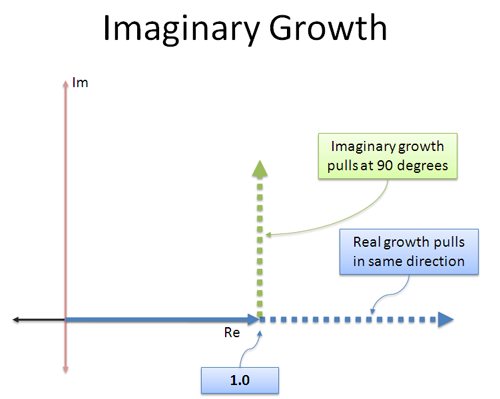
\includegraphics[scale=.6]{kait_image4}
  \end{center}
  \caption{Graph of imaginary growth.}
  \label{fig:4}
\end{figure}

Now let’s look at the most common definition of $e$:
\[e=\lim_{n\to\infty} (1+\frac{1}{n})^n\]

Here, $\frac{1}{n}$ represents the interest earned in an infinitesimal period as $x$ approaches infinity. But this assumes the interest is real. Let’s see what it would look like if it were imaginary:
\[e=\lim_{n\to\infty} (1+\frac{1 \cdot i}{n})^n\]

%Fifth image here (source: https://betterexplained.com/articles/intuitive-understanding-of-eulers-formula/)
\renewcommand{\thefigure}{5}
\begin{figure}[h]
  \begin{center}
    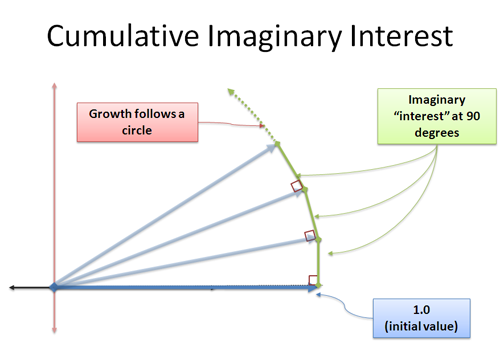
\includegraphics[scale=.6]{kait_image5}
  \end{center}
  \caption{Growth of imaginary "interest".}
  \label{fig:5}
\end{figure}

We can see that this imaginary growth begins to bring the point in a circle where $e^{ix}$ compounds itself by pulling in 90$^{\circ}$ increments as $n$ approaches infinity. This complex growth creates a complex unit circle. But why is it $e^{ix}$? Couldn’t the base be any other number? Well the answer comes in the derivative of $e^{ix}$.
\begin{center}
If $y=e^{ix}$, then $\frac{dy}{dx}=ie^{ix}$

For $x=0$, $e^{ix}=1$ and $ie^{ix}=i$.
\end{center}

This means the tangent line to $e^{ix}$ at $0$ is $i$. Let’s graph this. 

%Sixth image here (screenshotted from google doc)
\renewcommand{\thefigure}{6}
\begin{figure}[h]
  \begin{center}
    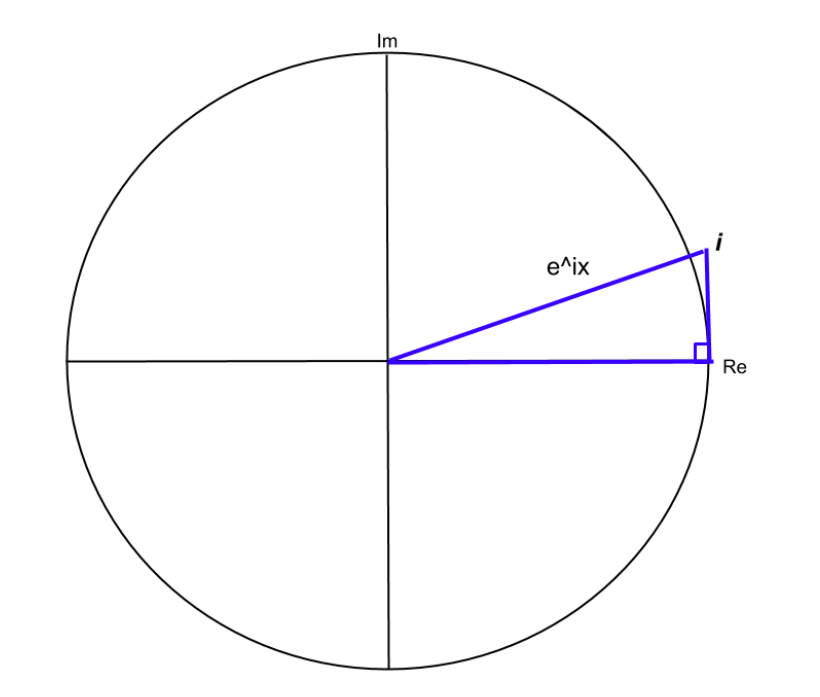
\includegraphics[scale=.3]{kait_image6}
  \end{center}
  \caption{Graph of tangent line to $e^{ix}$ at $0$.}
  \label{fig:6}
\end{figure}

Now we can see where the complex unit circle comes from. As $i$ is continuously compounded, it pulls at 90$^{\circ}$ until the unit circle is created. Now we know how $e^{ix}$ factors into the geometric interpretation of the formula. 

%Seventh image here (screenshotted from google doc)
\renewcommand{\thefigure}{7}
\begin{figure}[h]
  \begin{center}
    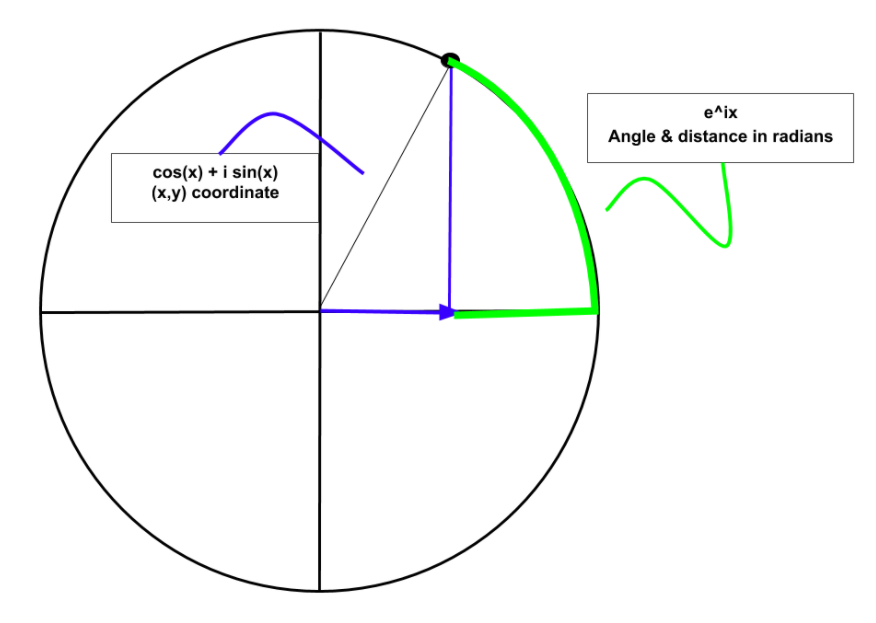
\includegraphics[scale=.3]{kait_image7}
  \end{center}
  \caption{Definition of the complex unit circle.}
  \label{fig:7}
\end{figure}

Here we can see how a single point on the complex unit circle (or complex plane using a constant $k$ as shown earlier) can be described in two ways. The first is with the cosine and complex sine of the point ($(x,y)$ coordinate) and as the complex growth of the radian ($e^{ix}$).

\noindent
\textbf{Remarks}

These four proofs are several of many proofs of Euler’s formula. Other proofs arise from group theory, vector calculus, derivatives, complex analysis, logarithms, and more. The true beauty of this concept is in the relationships between real numbers, complex numbers, Euler’s number, and complex exponents, in addition to its omnipresence within countless fields of mathematics. Furthermore, it links algebra, trigonometry, geometry, and even calculus together in a seamless fashion. It is also important to note the importance of complex numbers, which are often overlooked in standard algebra or pre-calculus courses, yet play a significant role in both physics and many areas of mathematics. Last, Euler’s formula is an example of a larger importance in mathematics: it may be a challenging concept to fully grasp, but the fact that there are so many ways by which to understand or think about it leads us to the notion that the true beauty of academics is the connections between thoughts, concepts, and ideas. The ability to understand concepts in multiple ways and make connections between various ideas is fundamental to academic growth and maturity. 

I will end with a question: How can Euler’s formula be used to solve something like $i^i$?